\chapter{Implementacija i korisničko sučelje}


\section{Korištene tehnologije i alati}

Frontend aplikacije realiziran je pomoću \href{https://reactjs.org}{Reacta} korištenjem programskog jezika \href{https://www.javascript.com/}{Javascript}.  React je Javascript biblioteka otvorenog koda za izgradnju korisničkih sučelja temeljenih na komponentama korisničkog sučelja. Backend aplikacije ostvaren je pomoću \href{https://spring.io/projects/spring-boot/}{Spring Boota} zasnovanog na razvojnom okviru \href{https://spring.io}{Spring}, pisanog u programskom jeziku \href{https://www.java.com/en/}{Java}. Od razvojnih okolina korišteni su \href{https://code.visualstudio.com/}{Visual Studio Code} i \href{https://www.jetbrains.com/idea/}{IntelliJ IDEA}. Pri uspostavi arhitekture su također korišteni \href{https://render.com/}{Render}, \href{https://www.netlify.com/}{Netlify}, \href{https://tailwindcss.com/}{Tailwind CSS}, \href{https://docs.docker.com}{Docker Docs}, \href{https://axios-http.com/}{Axios}, \href{https://reactrouter.com/en/main}{React-Router-Dom} i \href{https://www.google.com/recaptcha/}{reCAPTCHA}. Baza podataka pisana je u \href{https://www.postgresql.org/}{PostgreSQL}. Za komunikaciju, dogovore i sastanke korišteni su \href{https://web.whatsapp.com/}{WhatsApp}, \href{https://www.microsoft.com/en-us/microsoft-teams/log-in}{Microsoft Teams} te \href{https://start.atlassian.com/}{Atlassian}. \href{https://www.lucidchart.com/pages/}{Lucidchart} je alat korišten za kreiranje dijagrama, a sama dokumentacija je pisana u markup jeziku \href{https://www.latex-project.org}{LaTeX} te uz pomoć alata \href{https://www.overleaf.com/}{Overleaf}. Udaljeni repozitorij projekta smješten je na web platformi \href{https://github.com/}{GitHub}.


\eject 


\section{Ispitivanje programskog rješenja}

U ovom poglavlju provedeno je ispitivanje implementiranih funkcionalnosti na razini komponenti, s fokusom na ispitivanje jedinica (unit testing). Razrađeno je 6 ispitnih slučajeva koji obuhvaćaju redovne slučajeve, rubne uvjete, izazivanje pogrešaka (exception throwing) te ispitivanje neispravnog formata podataka.

\subsubsection{Ispitni slučaj 1: Redovni slučaj}
Opis: provjera ispravnog izvođenja osnovne funkcionalnosti. Unosi se nova soba.

\begin{figure}[H]
	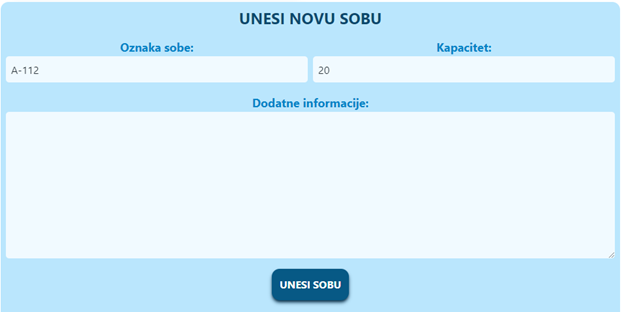
\includegraphics[scale=0.8]{slike/test1.png}
	\centering
	\caption{Test 1: Redovni slučaj}
	\label{fig:test1}
\end{figure}

Nova soba je uspješno dodana.

\begin{figure}[H]
	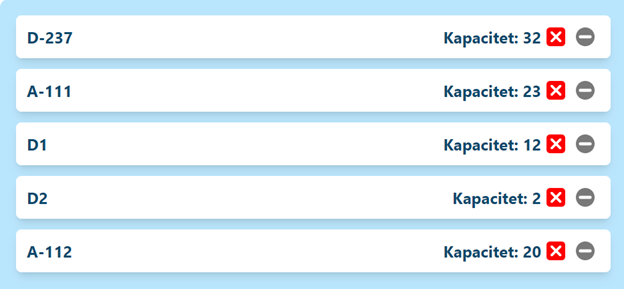
\includegraphics[scale=0.6]{slike/rez1.png}
	\centering
	\caption{Rezultat testa 1: Redovni slučaj}
	\label{fig:rez1}
\end{figure}

\subsubsection{Ispitni slučaj 2: Rubni uvjet}
Opis: ispitivanje ponašanja sustava kada su ulazni podaci na granici dopuštenih vrijednosti. Unosi se kapacitet sobe s minimalnom vrijednosti.

\begin{figure}[H]
	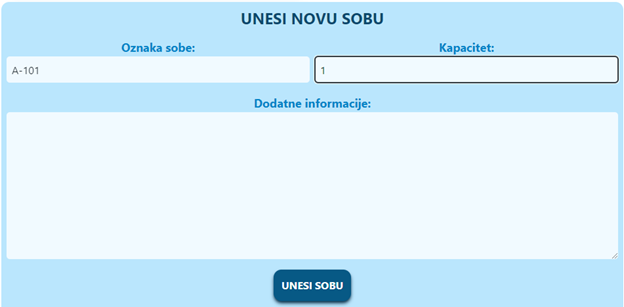
\includegraphics[scale=0.8]{slike/test2.png}
	\centering
	\caption{Test 2: Rubni uvjet}
	\label{fig:test2}
\end{figure}

Nova soba je uspješno dodana.

\begin{figure}[H]
	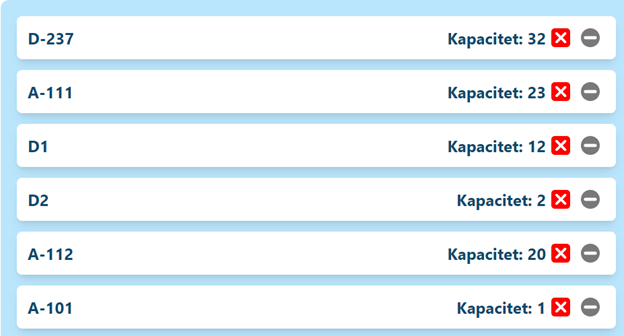
\includegraphics[scale=0.8]{slike/rez2.png}
	\centering
	\caption{Rezultat testa 2: Rubni uvjet}
	\label{fig:rez2}
\end{figure}

\eject

\subsubsection{Ispitni slučaj 3: Izazivanje pogrešaka}
Opis: provjera kako sustav reagira na izazivanje pogreške. Dodaje se soba s kapacitetom 0.

\begin{figure}[H]
	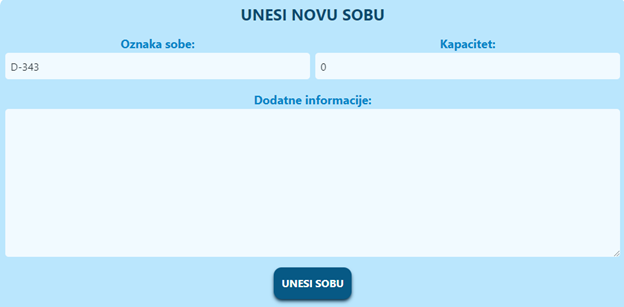
\includegraphics[scale=1]{slike/test3.png}
	\centering
	\caption{Test 3: Izazivanje pogrešaka}
	\label{fig:test3}
\end{figure}

Soba nije dodana i iskače poruka o pogrešci. 

\begin{figure}[H]
	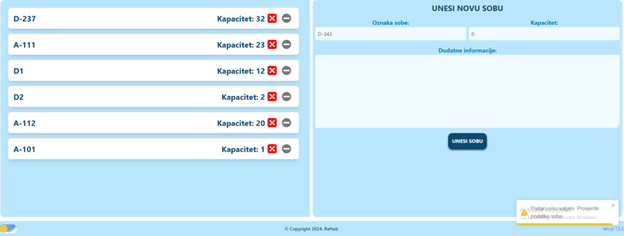
\includegraphics[scale=1]{slike/rez3.png}
	\centering
	\caption{Rezultat testa 3: Izazivanje pogrešaka}
	\label{fig:rez3}
\end{figure}

\eject

\subsubsection{Ispitni slučaj 4: Ispitivanje neispravnog formata podataka}
Opis: unos podataka u pogrešnom formatu. Unosi se zaposlenik s OIB-om u pogrešnom formatu.

\begin{figure}[H]
	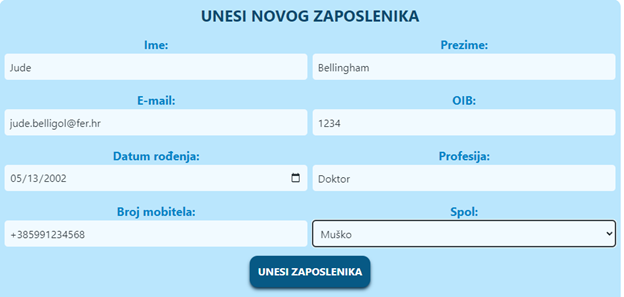
\includegraphics[scale=1]{slike/test4.png}
	\centering
	\caption{Test 4: Ispitivanje neispravnog formata podataka}
	\label{fig:test4}
\end{figure}

Nije dodan zaposlenik i iskače poruka o pogrešci. 

\begin{figure}[H]
	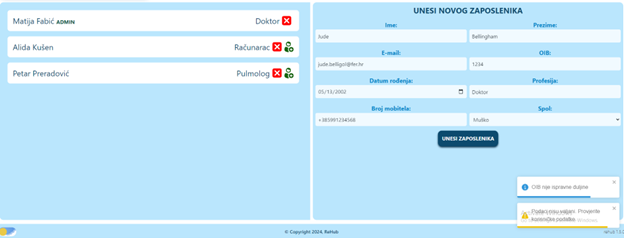
\includegraphics[scale=1]{slike/rez4.png}
	\centering
	\caption{Rezultat testa 4: Ispitivanje neispravnog formata podataka}
	\label{fig:rez4}
\end{figure}

\eject

\subsubsection{Ispitni slučaj 5: Ispitivanje neispravnog formata podataka}
Opis: unos podataka u pogrešnom formatu. Unosi se broj mobitela u pogrešnom formatu. 

\begin{figure}[H]
	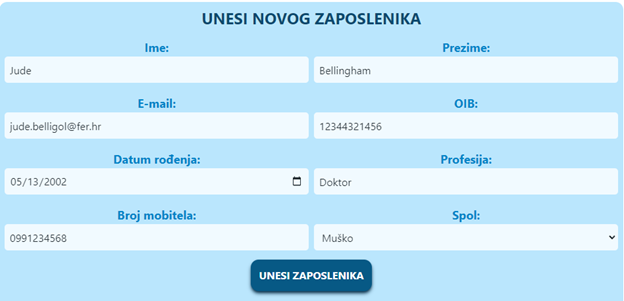
\includegraphics[scale=1]{slike/test5.png}
	\centering
	\caption{Test 5: Ispitivanje neispravnog formata podataka}
	\label{fig:test5}
\end{figure}

Nije dodan zaposlenik i iskače poruka o pogrešci. 

\begin{figure}[H]
	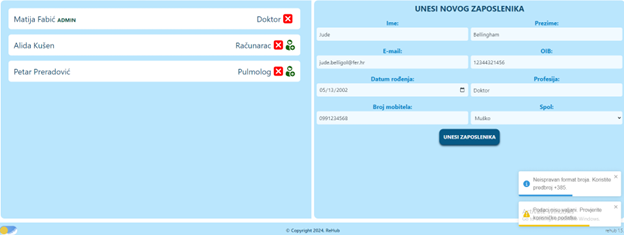
\includegraphics[scale=1]{slike/rez5.png}
	\centering
	\caption{Rezultat testa 5: Ispitivanje neispravnog formata podataka}
	\label{fig:rez5}
\end{figure}

\eject

\subsubsection{Ispitni slučaj 6: Ispitivanje neispravnog formata podataka}
Opis: unos podataka u pogrešnom formatu. Kao kapacitet sobe unose se slova.  

\begin{figure}[H]
	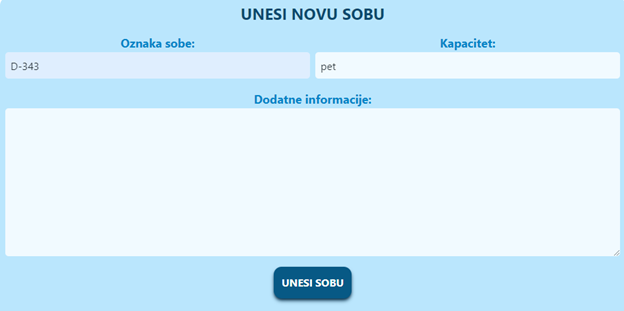
\includegraphics[scale=1]{slike/test6.png}
	\centering
	\caption{Test 6: Ispitivanje neispravnog formata podataka}
	\label{fig:test6}
\end{figure}

Nije dodana soba i iskače poruka o pogrešci. 

\begin{figure}[H]
	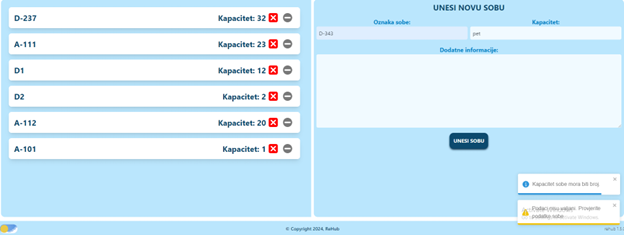
\includegraphics[scale=1]{slike/rez6.png}
	\centering
	\caption{Rezultat testa 6: Ispitivanje neispravnog formata podataka}
	\label{fig:rez6}
\end{figure}



\eject 


\section{Dijagram razmještaja}

Dijagram razmještaja opisuje strukturu sustava, tj. odnose između sklopovskih i programskih dijelova. Donja slika predstavlja specifikacijski dijagram razmještaja, pri čemu se na poslužiteljskom računalu nalaze web aplikacija i baza podataka. Pristup aplikaciji klijenti ostvaruju putem web preglednika. Funkcioniranje sustava temelji se na modelu "klijent - poslužitelj", gdje klijenti zahtijevaju usluge od poslužitelja putem HTTP zahtjeva te očekuju odgovor. Poslužitelj obrađuje zahtjeve i šalje odgovore klijentima, a istovremeno upravlja komunikacijom s bazom podataka.

\begin{figure}[H]
	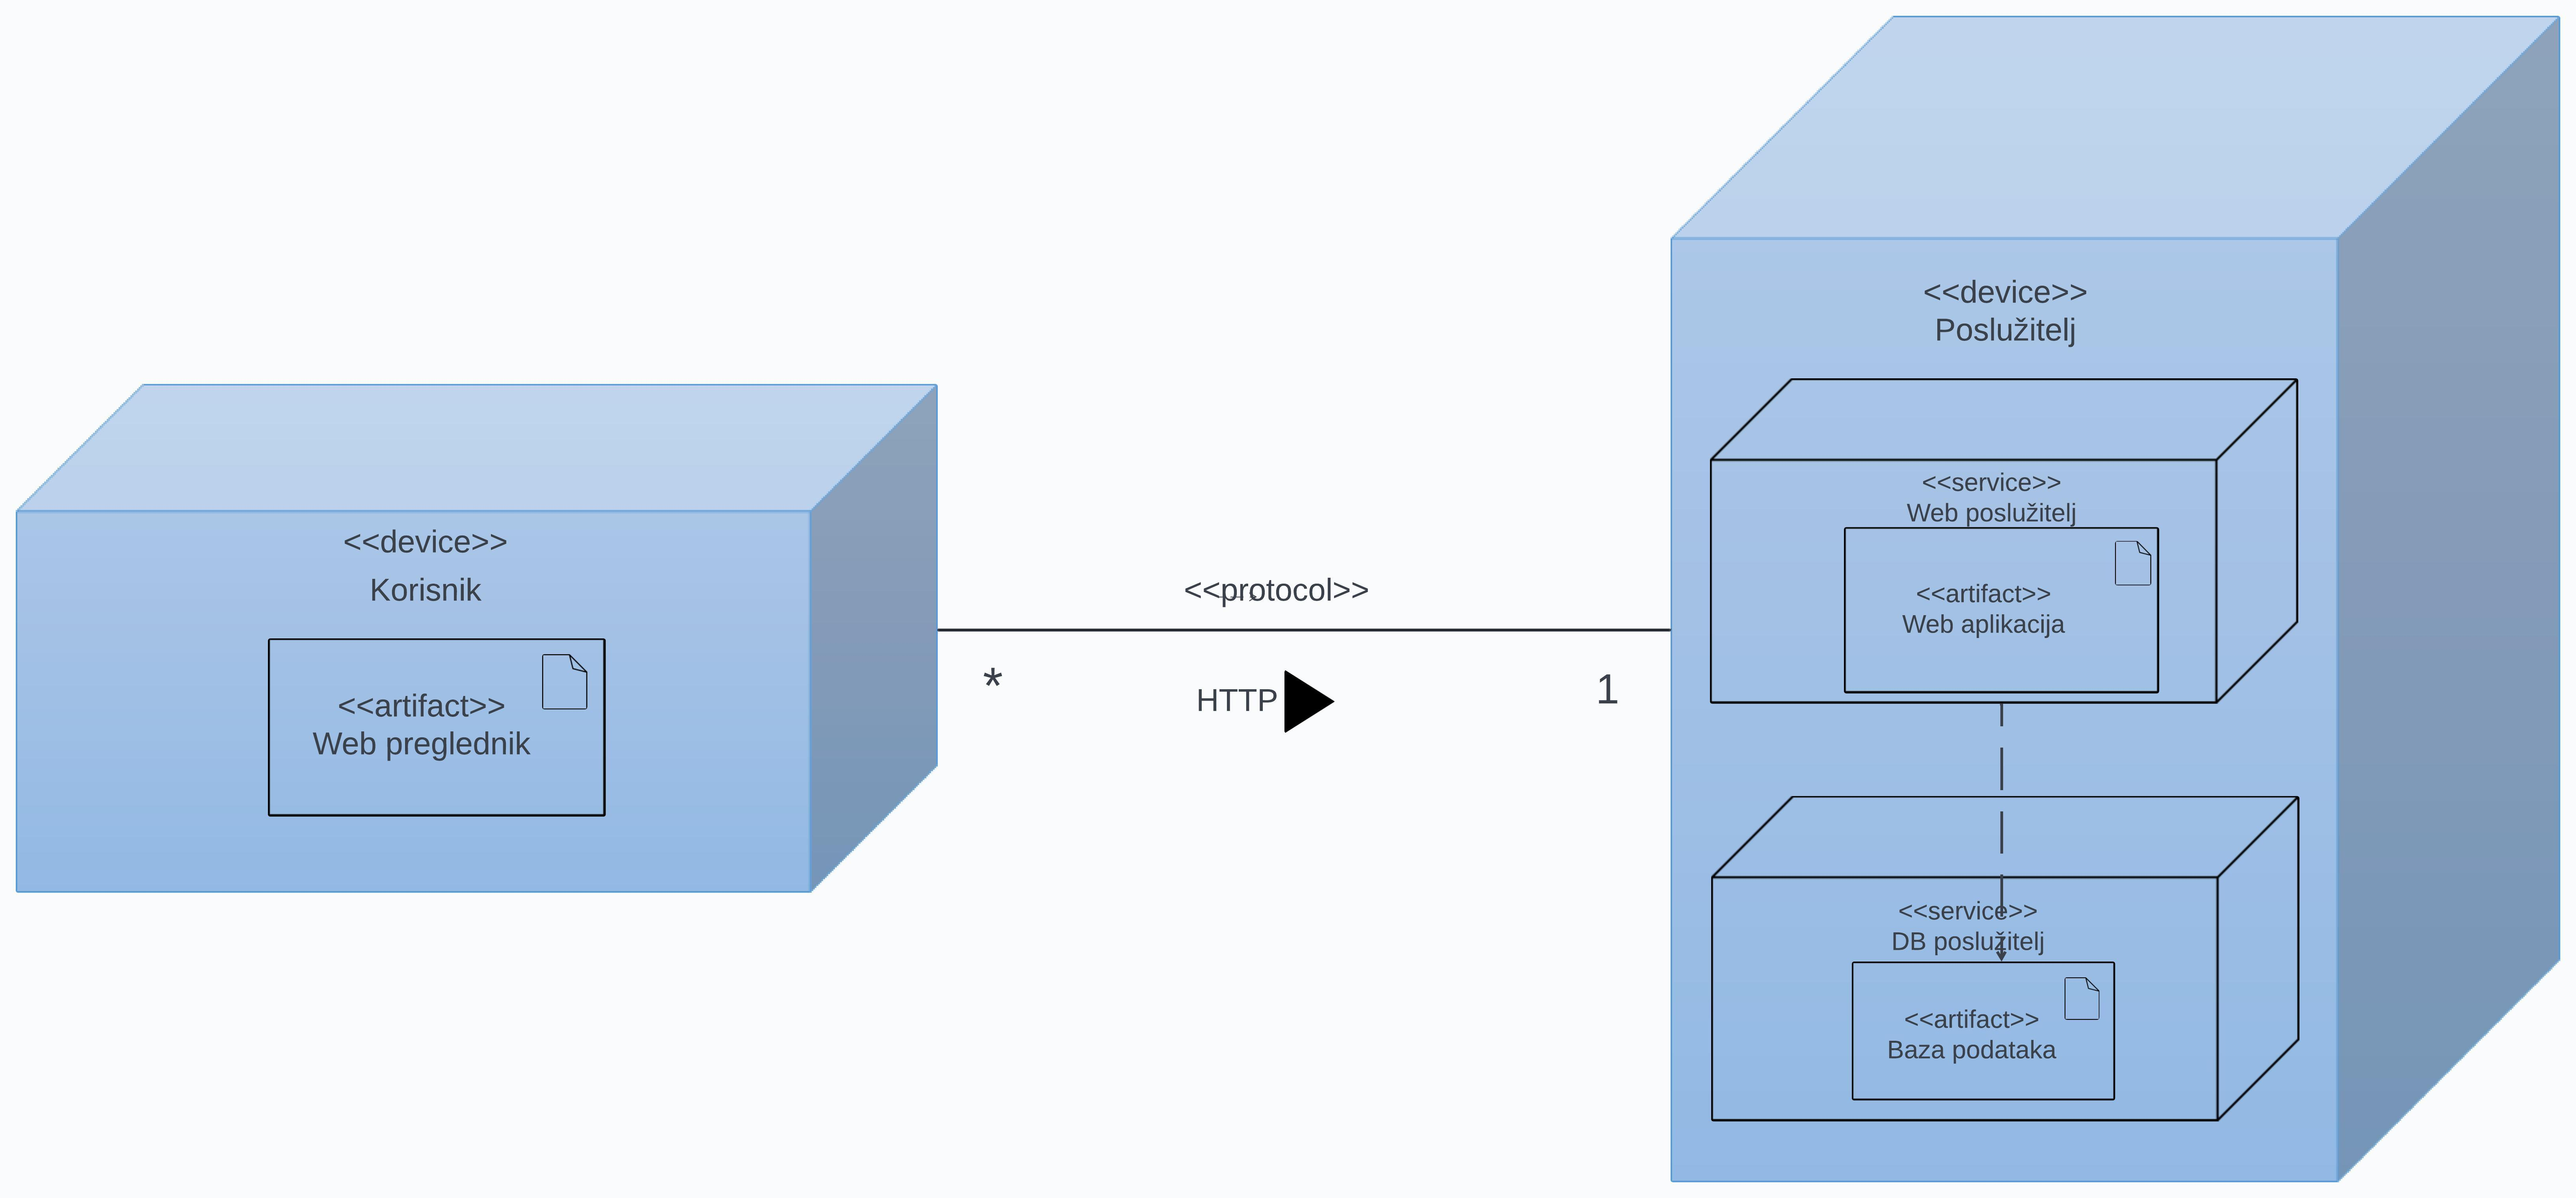
\includegraphics[scale=0.15]{dijagrami/Layout Diagram.jpeg}
	\centering
	\caption{Specifikacijski dijagram razmještaja}
	\label{fig:LayoutDiagram}
\end{figure}

\eject 

\section{Upute za puštanje u pogon}

Aplikacija je uspješno implementirana i dostupna na platformi Netlify. Za poslužitelj backend-a koristi se alat Render. Kako bi iskoristili sve korisne značajke koje Render pruža, potrebno je stvoriti instance baze podataka, poslužitelja za backend, te poslužitelja za frontend aplikacije. Prvi korak je kreiranje PostgreSQL baze podataka.

\begin{figure}[H]
	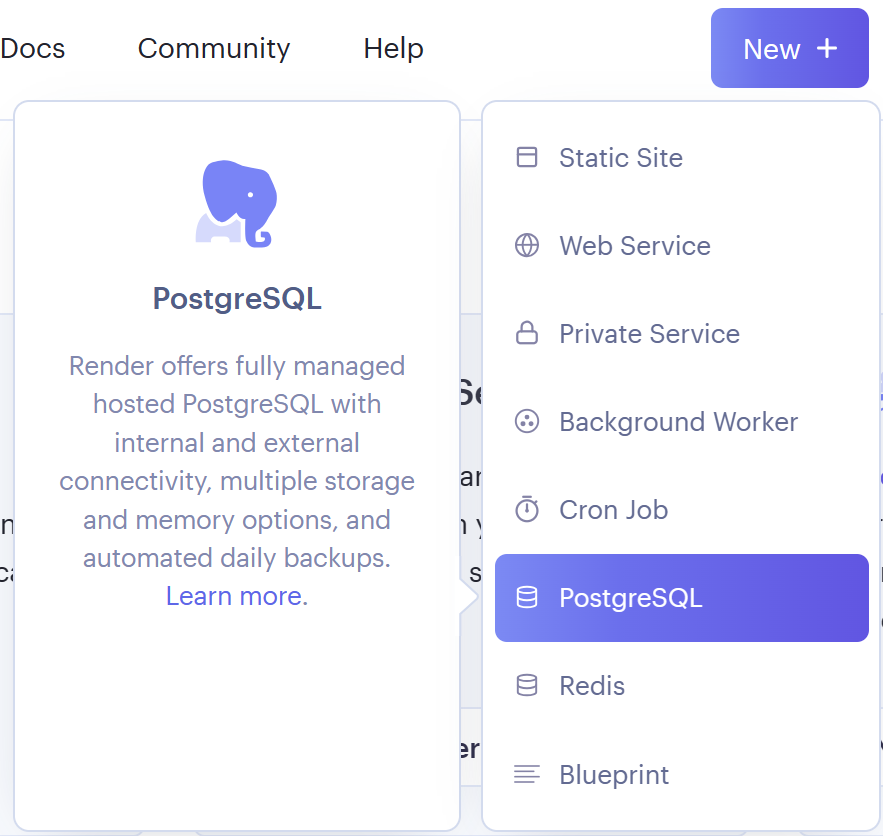
\includegraphics[scale=0.7]{dijagrami/PostgresSQL.png}
	\centering
	\caption{Izbornik za stvaranje nove baze podataka}
	\label{fig:PostgresSQL}
\end{figure}



Potrebno je upisati ime baze, odabrati regiju poslužitelja instance i označiti tip instance koji će se koristiti.

\begin{figure}[H]
	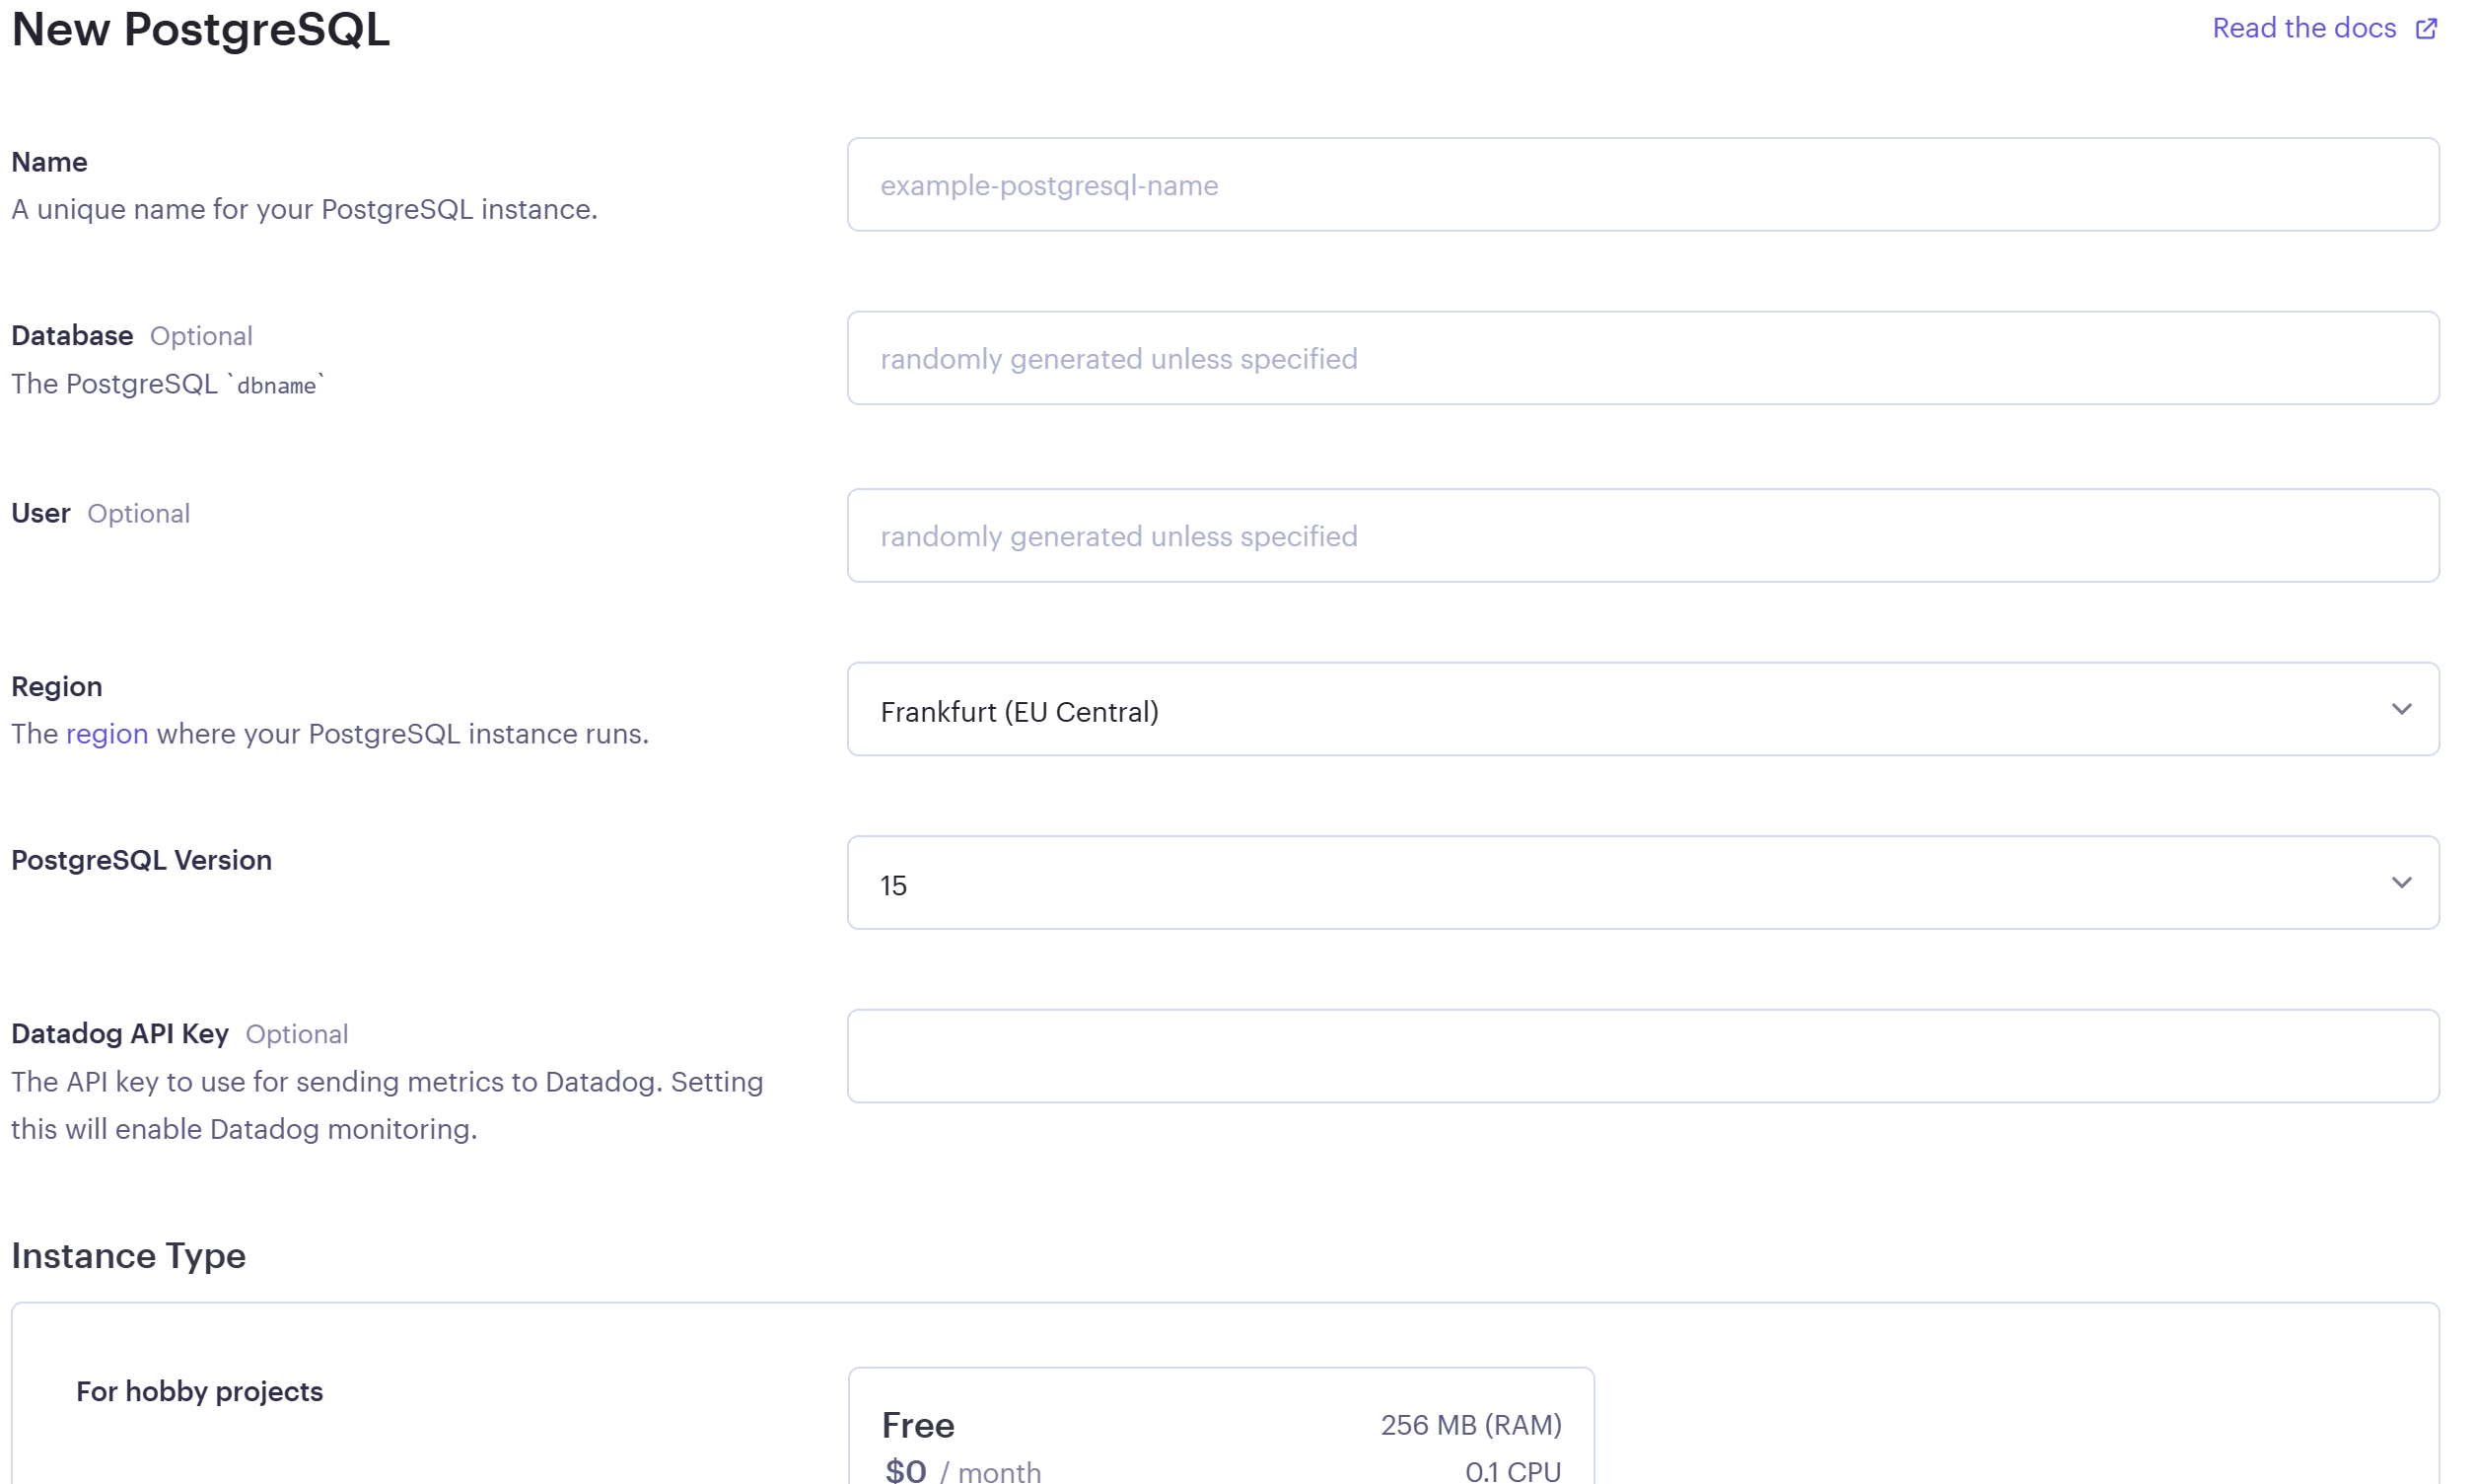
\includegraphics[scale=0.4]{dijagrami/stvaranje-baze.png}
	\centering
	\caption{Stvaranje nove baze podataka}
	\label{fig:tvaranje-baze}
\end{figure}



Nakon ovih koraka treba pokrenuti stvaranje pritiskom na tipku ”Create”.
Pokazuje se prozor u kojemu su navedeni osnovni podaci o bazi kao ime, verzija, regija, prostor za pohranu, API ključ, itd.
Kad je baza uspješno kreirana, potrebno je uzeti podatke koje treba dati backendu aplikacije. Ti podatci se nalaze u poljima \textit{Hostname}, \textit{Port}, \textit{Database}, \textit{Username}, \textit{Password} i \textit{External Database URL}.



Backend je implementiran na Render platformi, koristeći Docker slike koje se automatski generiraju i implementiraju prilikom svakog push-a na master granu. Proces implementacije upravlja se pomoću GitHub Actions radnog toka definiranog u datoteci \textit{build-test-deploy.yaml}, koji obuhvaća korake poput preuzimanja koda, postavljanja JDK 17, izgradnje, testiranja, kopiranja JAR datoteke i prijenosa artefakta. Docker slika se označava tijekom procesa izgradnje. 

\begin{figure}[H]
	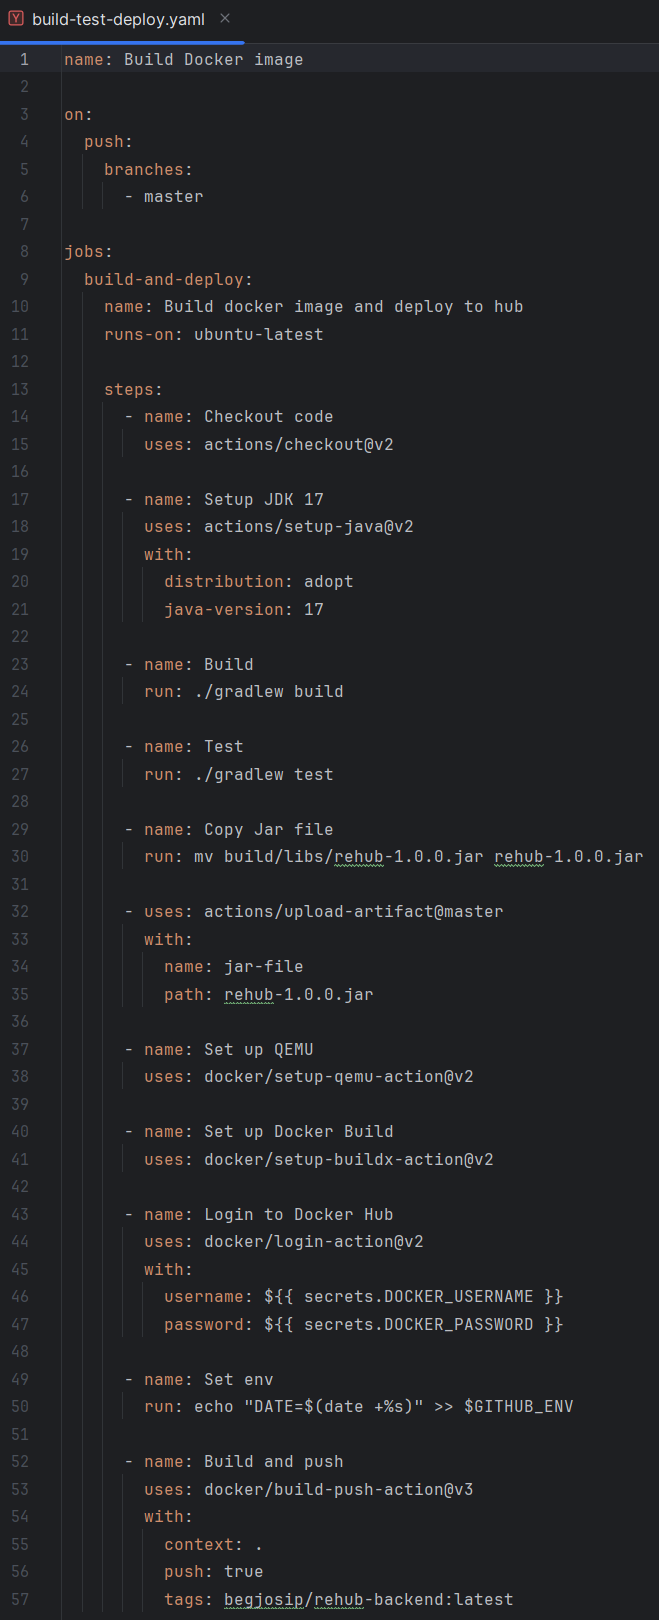
\includegraphics[scale=0.5]{dijagrami/built-test-deploy.png}
	\centering
	\caption{Datoteka \textit{Datoteka build-test-deploy}}
	\label{fig:built-test-deploy}
\end{figure}



Konfiguracija backend-a upravlja se putem datoteke \textit{application-prod.properties}, koja sadrži ključne parametre za konfiguraciju poslužitelja, prijenosa datoteka, podatkovnog izvora, e-pošte, ponovnog postavljanja lozinke, provjere korisnika, JPA i Flyway konfiguraciju te Jackson konfiguraciju. Svi ovi parametri su pažljivo prilagođeni kako bi podržali funkcionalnosti i integracije aplikacije, čime se osigurava glatki i učinkoviti razvojni i implementacijski proces backend-a.

\begin{figure}[H]
	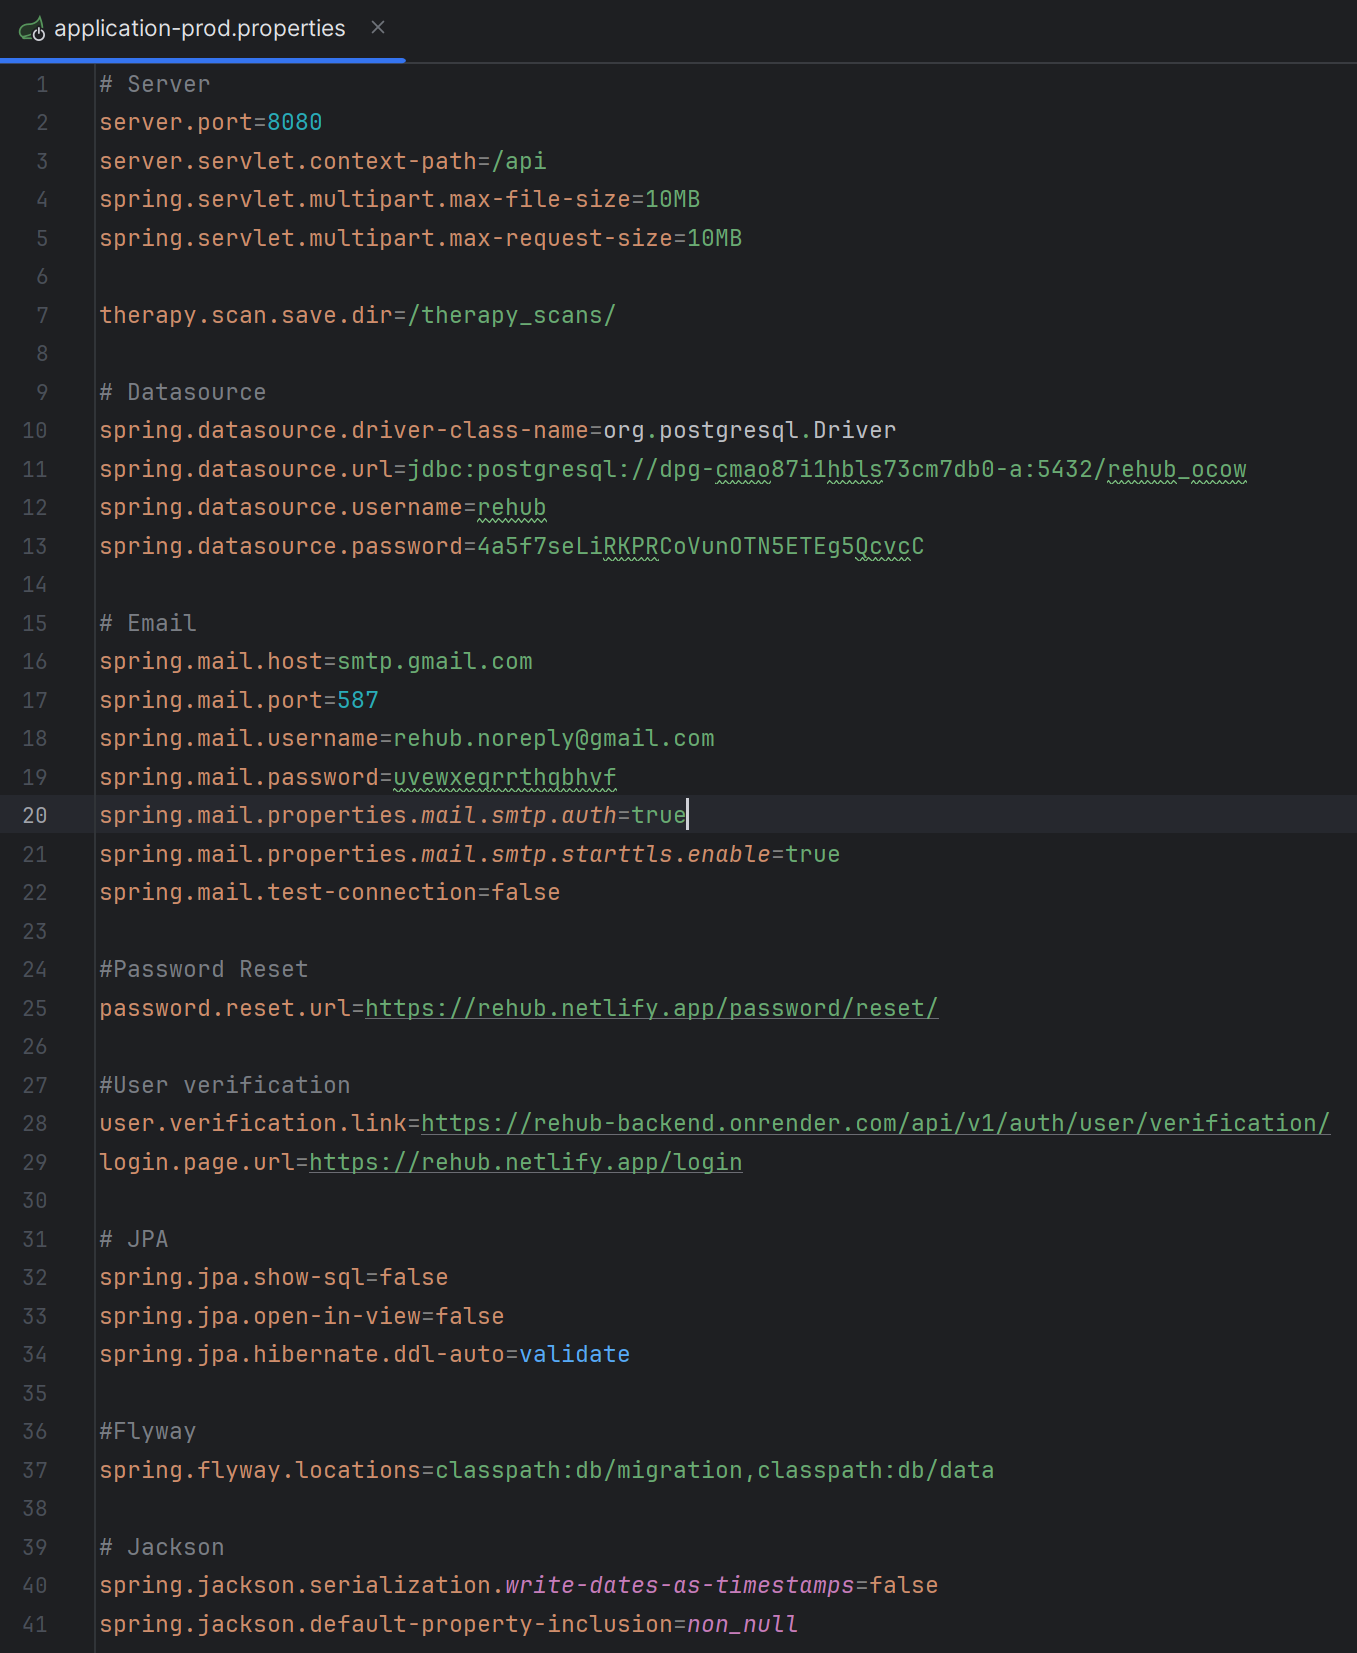
\includegraphics[scale=0.6]{dijagrami/app-prod.png}
	\centering
	\caption{Datoteka \textit{application-prod.properties}}
	\label{fig:app-prod}
\end{figure}



URL backend-a: https://rehub-backend.onrender.com/



Frontend aplikacija je postavljena za automatski deploy na Netlify prilikom push-a na master granu. U datoteci \textit{build-deploy.yaml} specificiran je GitHub Actions radni tok za deploy na Netlify. 	

\begin{figure}[H]
	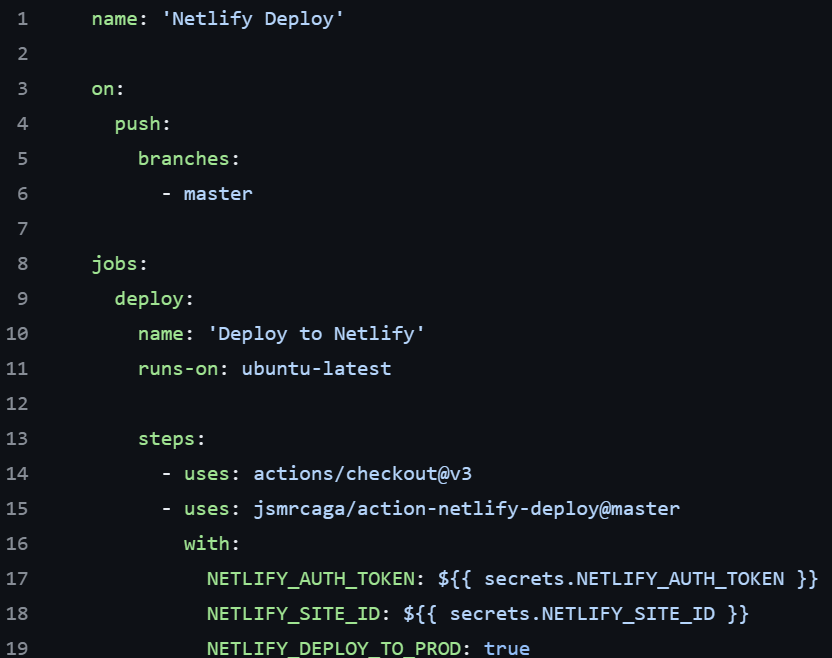
\includegraphics[scale=0.9]{dijagrami/bulid-and-deploy.png}
	\centering
	\caption{Datoteka \textit{build-and-deploy.yaml}}
	\label{fig:build-and-deploy}
\end{figure}



U Netlify konzoli, u postavkama projekta, konfigurirajte \textit{build} opcije.

\begin{figure}[H]
	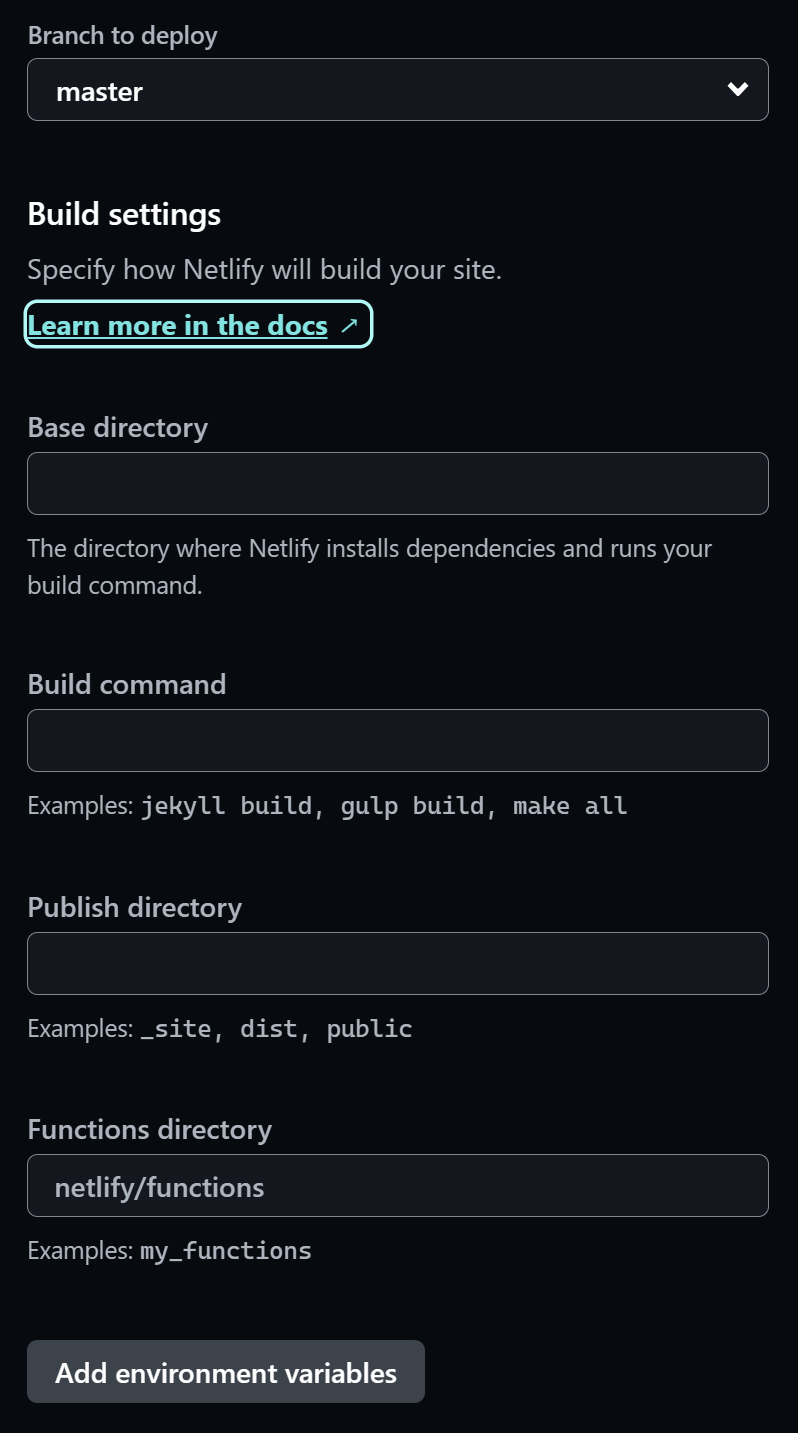
\includegraphics[scale=0.7]{dijagrami/netlify-conf.png}
	\centering
	\caption{Postavljanje konfiguracije}
	\label{fig:netlify-conf}
\end{figure}

\textit{Base Directory}: Postavite na direktorij u kojem se nalazi package.json.
\textit{Build Command}: Postavite na naredbu koja pokreće izgradnju projekta, u ovom slučaju npm run build.
\textit{Publish Directory}: Odredite direktorij koji sadrži izgrađene artefakte, u ovom slučaju build.



Aplikacija je puštena u pogon i spremna za uporabu. Pristupa se preko adrese koja je navedena za instancu frontenda.
https://rehub.netlify.app

\eject